This section contains the main problem for this project and the form of solution required.

\subsection{The problem}
The analysis was based on the initial problem: \textit{How can the current \citybike system be improved, in order to make it more usable?}.
From the analysis, it was found that the current \citybike has several problems, limiting the overall usability (as described in \cref{aalborg_bycyklen:challenges}).

The main problems identified were:
\begin{itemize}
\item Missing bikes (Left outside stations)
\item Flexibility (No certainty when going to station, or when a bike will be available)
\item Reliability (No lock for short stops)
\item Broken bikes (Possibly left for a long time)
\end{itemize}

Additionally, certain limitations were set by Aalborg Kommune, collected through the interview:

\begin{itemize}
\item Simplicity (No renting/booking)
\end{itemize}

\subsection{Scope}
Due to the size of the problems described, as well as the limitations asserted by Aalborg Kommune, the following problem has will not be handled by this project: \textbf{Reliability}.

Solving this problem is relying on a more complex locking system for the bikes, which is more interesting from a hardware perspective, but not as much from a software perspective.
\mikael{Is this crazy?}

\subsection{Solution}
The biggest change to the current system, will be the addition of GPSs in the bikes.
This will provide the following opportunities:
\begin{itemize}
\item It will be possible to track the position of bikes.
\item Bike stations will be completely obsolete, instead 'hot-spots' will be introduced.
\item It will be possible to monitor the usage of bikes, thus statistical predictions on future locations and behavior will be possible.
\end{itemize}

\paragraph{Bike stations are unnecessary}
So far, bike stations serve a limited purpose.
They are where people are supposed to place the bikes after use, thus making it possible for other people to find the bikes.
However, bikes are not necessarily returned to a station after use, somewhat disrupting the sole purpose of the bike stations.

\paragraph{GPS}
Furthermore, by adding GPSs to the bikes, it will be possible to get an exact location of a bike, even if it is not at a bike station.
By monitoring the location of the bikes, their movements could be tracked.
Further, by detecting long stops (meaning ended trip), so-called hot-spots could be determined.

\paragraph{Hot-spot}
A hot-spot is an area, like an informal station.
But hot-spots come and go, depending on the use of the bikes.
A hot-spot is initialized when several bikes are available at the hot-spot location.
This is determined by looking at the history of the bike usage.

\paragraph{Locating bikes}
By requesting GPS locations from the bikes, it will be possible to get an overview of all available bikes.

\paragraph{Structure of the solution}
The structure of the solution can be seen in \cref{fig:solution_structure}.
The figure illustrates the software systems running on a server and what each system interact with.
 
\begin{figure}[h]
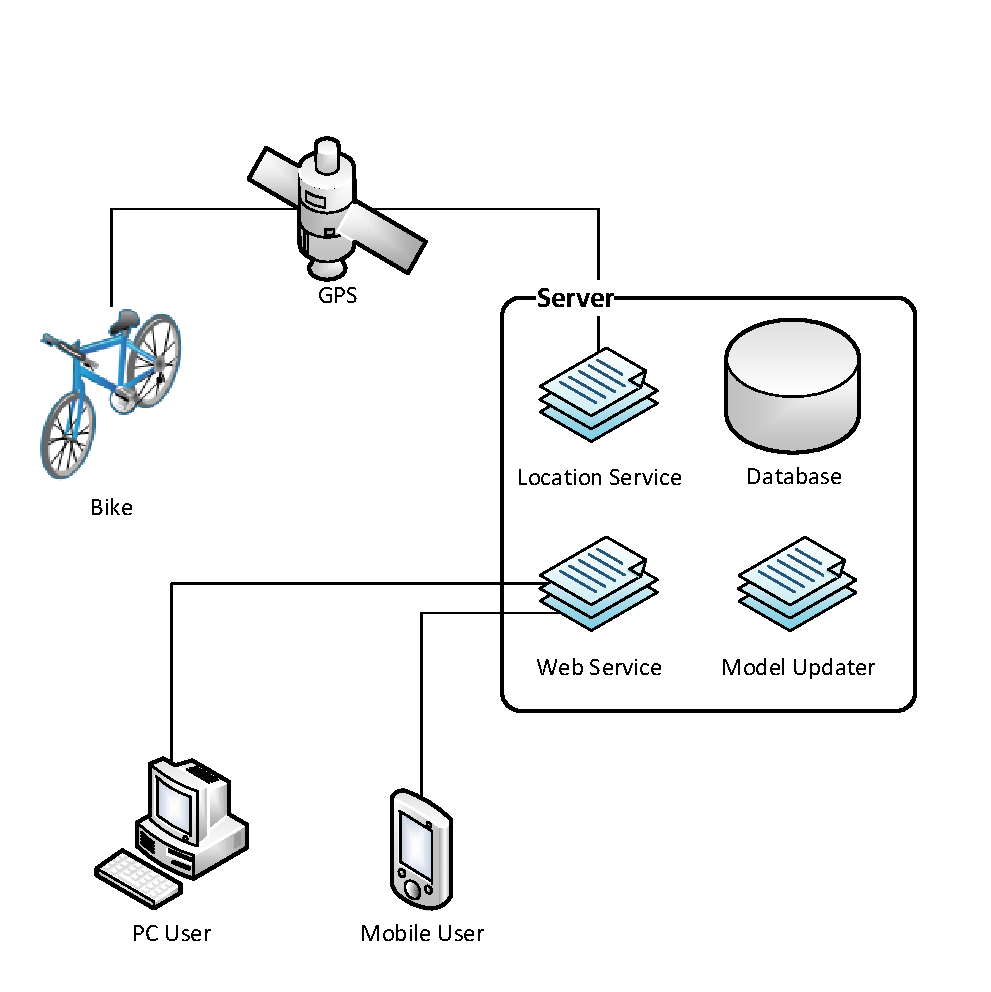
\includegraphics[width=\textwidth]{our_solution.pdf}
\caption{The overall structure of our solution}
\label{fig:solution_structure}
\end{figure}

The location service continuously request GPS data from the bikes and stores it in the database.

The web service handles requests from the users and returns a result based on the data in the database.

The inactivity agent continuously look in the database to check if a bike has been inactive for too long, then notifies Aalborg Kommune.